V programih pogosto želimo nek seznam števil urediti po vrsti.
V ta namen lahko napišemo svojo funkcijo, ki implementira enega od znanih
algoritmov za urejanje; npr.~\emph{bubble sort}, \emph{insertion sort},
\emph{quick sort}, ipd.
Ker pa so učinkovite implementacije pogosto komplicirane in se pri pisanju hitro
zmotimo, je bolje, da uporabimo funkcije, ravno v ta namen vključene v
standardno knjižnjico.
Za to bomo potrebovali na začetek programa dodati še dve vrstici:

\fkoda{poglavja/urejanje/algorithm.cpp}

Ukaz \verb+#include+ že poznamo, opazimo pa, da tokrat za spremembo nima končnice
\koda{.h}.
To je zato, ker funkcije, ki smo jih uporabljali do sedaj, izvirajo iz jezika C,
tokrat pa potrebujemo funkcijo, napisano posebaj za C++.
To razloži tudi drugo vrstico; vse funkcije v standardni knjižnjici v C++ so
vključene v imenski prostor \koda{std}.
Če jih želimo klicati, moramo pred ime funkcije vedno napisati \koda{std::}, ali
pa na začetek programa vključiti vrstico \koda{using namespace std}.

Sedaj lahko uporabimo funkcijo \koda{sort}, ki sprejme dva argumenta;
kazalec na začetek in tik za konec predela spomina, ki ga želimo urediti.
Poglejmo si enostavni primer.

\fkoda{poglavja/urejanje/uporaba.cpp}

Program prebere število $n$, za njim pa še $n$ števil, jih uredi naraščajoče,
in jih izpiše.
Funkcijo \koda{sort} smo poklicali tako, da smo kot prvi argument podali seznam
\koda{arr} (oz.~kazalec na prvi element seznama), kot drugi argument pa kazalec
na prvo mesto v spominu, ki ne spada več v naš seznam (oz.~prvo mesto v spominu,
ki ga ne želimo urediti).
Na primer, če želimo urediti seznam \koda{arr} z $10$ elementi, moramo podati
kazalca \koda{arr} in \koda{arr+10}, kot je prikazano spodaj:

\begin{figure*}[h!]
  \centering
  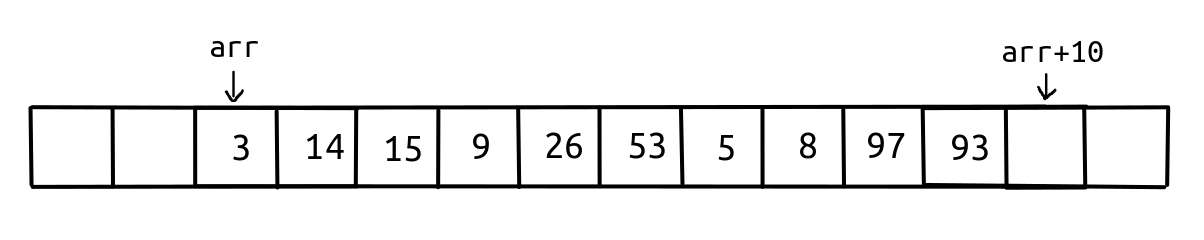
\includegraphics[width=0.9\textwidth]{poglavja/urejanje/addressing}
\end{figure*}

Optimalna časovna zahtevnost algoritma za urejanje je $O(n \log n)$.
To v praksi pomeni, da bo urejanje delovalo dovolj hitro za $n \le 10^6$
podatkov.
Če imamo več podatkov kot toliko, bo urejanje trajalo predolgo in naša rešitev
ne bo sprejeta.

\naslov{Primerjalna funkcija}

Če želimo urediti seznam padajoče namesto naraščajoče, lahko seznam prvo uredimo
naraščajoče, in ga nato obrnemo.
Ker s tem dobimo veliko dodatnega dela, je bolje, da funkciji \koda{sort} podamo
lastno primerjalno funkcijo.
Le-ta mora sprejeti dva argumenta ter vrniti \koda{bool}, in sicer; če mora biti
prvi argument v urejenem seznamu levo od drugega, mora funkcija vrniti \koda{true},
sicer pa \koda{false}.
Če ne podamo tretjega argumenta, se \koda{sort} obnaša tako, kot da bi podali
naslednjo funkcijo:

\fkoda{poglavja/urejanje/compare.cpp}

Če želimo urediti seznam padajoče, moramo torej le podati nasprotno funkcijo,
kot spodaj:

\fkoda{poglavja/urejanje/nasprotno.cpp}

\naslov{Urejanje sestavljenih podatkov}

Recimo, da imamo v nalogi dana imena tekmovalcev ter točke, ki so jih ti
tekmovalci dosegli na tekmovanju, naš cilj pa je, da izpišemo imena tekmovalcev
po vrsti glede na doseženo število točk.
Če bomo prebrali točke in imena v različna seznama, ter uredili seznam točk, bo
seznam imen ostal nespremenjen in ne bomo več vedeli, katero ime pripada katerim
točkam.

Kako uredimo oba seznama hkrati?
Najbolj enostavna možnost je uporaba \koda{struct}, ki pa ga še ne poznamo.
Namesto tega si lahko pripravimo seznam indeksov, ki na začetku na $i$-tem mestu
hrani številko $i$.
Potem sestavimo funkcijo \koda{compare} tako, da sprejme dva indeksa, ter ju uredi
glede na vrednosti v tabeli s točkami na pripadajočih indeksih.
Urejamo pa ne tabele s točkami, temveč novo tabelo indeksov.
Na ta način se tabeli s točkami in z imeni ne bosta spreminjali, in bodo točke
pripadale imenu na istem indeksu.

Primer implementacije opisane rešitve je prikazan spodaj.

\fkoda{poglavja/urejanje/kombinirani.cpp}

\noindent
Če programu podamo spodnji vhod,
\begin{verbatim}
5
France 37
Gregor 34
Julija 38
Matija 29
Urska 8
\end{verbatim}
nam bo izpisal imena, urejena padajoče po številu točk:
\begin{verbatim}
Julija
France
Gregor
Matija
Urska
\end{verbatim}